%\documentclass[12pt]{article}
%\usepackage{graphicx,psfrag,amsfonts,float,mathbbol,xcolor,cleveref}
%\usepackage{arydshln}
%\usepackage{amsmath}
%\usepackage{tikz}
%\usepackage[mathscr]{euscript}
%\usepackage{enumitem}
%\usepackage{accents}
%\usepackage{lscape}
%\usepackage{subcaption}
%\usepackage{longtable}
%\usepackage{framed}
%%\usepackage{subcaption}
%%\usepackage[hang]{subfigure}
%%\usepackage{subfig} 
%\usepackage{booktabs}
%\usepackage{natbib}
%\usepackage{mathtools}
%\usepackage{IEEEtrantools}
%\usepackage{times}
%\usepackage{filecontents}
%\usepackage{subfiles}
%\usepackage{cite}
%\usepackage{subcaption}
%\usepackage{rotating}
%\usepackage{arydshln}
%\usepackage{amsthm}
%\usepackage[letterpaper, left=1in, top=1in, right=1in, bottom=1in,nohead,includefoot, verbose, ignoremp]{geometry}
%\usepackage{booktabs}
%\newcommand{\ra}[1]{\renewcommand{\arraystretch}{#1}}
%\newcommand\numberthis{\addtocounter{equation}{1}\tag{\theequation}}
%\newcommand*\needsparaphrased{\color{red}}
%\newcommand*\needscited{\color{orange}}
%\newcommand*\needsproof{\color{blue}}
%\newcommand*\outlineskeleton{\color{green}}
%\newcommand{\PP}{\mathcal{P}}
%\newcommand{\hilbert}{\mathcal{H}}
%\newcommand{\hilbertl}{\mathcal{H}_{\langle l \rangle}}
%\newcommand{\hilbertm}{\mathcal{H}_{\langle m \rangle}}
%\newcommand{\hilbertlnull}{\mathcal{H}_{0\langle l \rangle}}
%\newcommand{\hilbertmnull}{\mathcal{H}_{0\langle m \rangle}}
%\newcommand{\hilbertlpen}{\mathcal{H}_{1\langle l \rangle}}
%\newcommand{\hilbertmpen}{\mathcal{H}_{1\langle m \rangle}}
%
%\newcommand{\bfeps}{\mbox{\boldmath $\epsilon$}}
%\newcommand{\bfgamma}{\mbox{\boldmath $\gamma$}}
%\newcommand{\bflam}{\mbox{\boldmath $\lambda$}}
%\newcommand{\bfphi}{\mbox{\boldmath $\phi$}}
%\newcommand{\bfsigma}{\mbox{\boldmath $\sigma$}}
%\newcommand{\bfbeta}{\mbox{\boldmath $\beta$}}
%\newcommand{\bfalpha}{\mbox{\boldmath $\alpha$}}
%\newcommand{\bfe}{\mbox{\boldmath $e$}}
%\newcommand{\bff}{\mbox{\boldmath $f$}}
%\newcommand{\bfone}{\mbox{\boldmath $1$}}
%\newcommand{\bft}{\mbox{\boldmath $t$}}
%\newcommand{\bfo}{\mbox{\boldmath $0$}}
%\newcommand{\bfO}{\mbox{\boldmath $O$}}
%\newcommand{\bfx}{\mbox{\boldmath $x$}}
%\newcommand{\bfX}{\mbox{\boldmath $X$}}
%\newcommand{\bfz}{\mbox{\boldmath $z$}}
%\newcommand{\argmin}[1]{\underset{#1}{\operatorname{arg}\,\operatorname{min}}\;}
%\DeclareMathAlphabet{\mathpzc}{OT1}{pzc}{m}{it}
%
%\newcommand{\bfm}{\mbox{\boldmath $m}}
%\newcommand{\bfy}{\mbox{\boldmath $y$}}
%\newcommand{\bfa}{\mbox{\boldmath $a$}}
%\newcommand{\bfb}{\mbox{\boldmath $b$}}
%\newcommand{\bfY}{\mbox{\boldmath $Y$}}
%\newcommand{\bfS}{\mbox{\boldmath $S$}}
%\newcommand{\bfZ}{\mbox{\boldmath $Z$}}
%\newcommand{\cardT}{\vert \mathcal{T} \vert}
%%\newenvironment{theorem}[1][Theorem]{\begin{trivlist}
%%\item[\hskip \labelsep {\bfseries #1}]}{\end{trivlist}}
%%\newenvironment{corollary}[1][Corollary]{\begin{trivlist}
%%\item[\hskip \labelsep {\bfseries #1}]}{\end{trivlist}}
%%\newenvironment{proposition}[1][Proposition]{\begin{trivlist}
%%\item[\hskip \labelsep {\bfseries #1}]}{\end{trivlist}}
%%\newenvironment{definition}[1][Definition]{\begin{trivlist}
%%\item[\hskip \labelsep {\bfseries #1}]}{\end{trivlist}}
%
%\newtheorem{theorem}{Theorem}[section]
%\newtheorem{lemma}[theorem]{Lemma}
%\newtheorem{proposition}[theorem]{Proposition}
%\newtheorem{corollary}[theorem]{Corollary}
%
%\theoremstyle{definition}
%\newtheorem{definition}{Definition}[section]
%\newtheorem{example}{Example}[section]
%\def\bL{\mathbf{L}}
%
%\begingroup\lccode`~=`_
%\lowercase{\endgroup\def~}#1{_{\scriptscriptstyle#1}}
%\AtBeginDocument{\mathcode`_="8000 \catcode`_=12 }
%\makeatletter
%\newcommand{\clearsubcaptcounter}{\setcounter{sub\@captype}{0}}
%\renewcommand{\theenumi}{\Roman{enumi}}
%\renewcommand{\labelenumi}{\theenumi.}
%\renewcommand{\theenumii}{\Alph{enumii}}
%\renewcommand{\labelenumii}{\theenumii.}
%\renewcommand{\p@enumii}{\theenumi.}
%\makeatother
%
%
%\DeclareCaptionSubType*[arabic]{table}
%\captionsetup[subtable]{labelformat=simple,labelsep=colon}
%\begin{document}
%
%%\nocite{*}
%\def\bL{\mathbf{L}}
%%\usepackage{mathtime}
%
%%%UNCOMMENT following line if you have package
%
%
%\title{ Nonparametric Covariance Estimation for Longitudinal Data via Penalized Tensor Product Splines}
%
%\author{Tayler A. Blake\thanks{The Ohio State University, 1958 Neil Avenue, Columbus, OH 43201} \and  Yoonkyung Lee\thanks{The Ohio State University, 1958 Neil Avenue, Columbus, OH 43201}}
%
%\bibliographystyle{plainnat}
%\maketitle

\chapter{Simulation studies} 
\section{Performance benchmarking with complete data}

In this section we compare bivariate spline estimators of the Cholesky factor to other methods of covariance estimation. Our primary comparisons are that with the parametric polynomial estimator proposed by \cite{pourahmadi1999joint},  \cite{pan2003modelling}, and \cite{pourahmadi2002dynamic}, which is also based on the modified Cholesky decomposition, and with the oracle estimator, which effectively gives a lower bound on the risk for given covariance structure. As a benchmark, we also include the sample covariance matrix, and two regularized variants of it: the tapered sample covariance matrix (\cite{cai2010optimal}) and the soft thresholding estimator (\cite{rothman2009generalized}), which does not rely on a natural ordering among the variables. In the simulations, the smoothing spline estimator of the modified Cholesky decomposition was constructed using the framework of a tensor product cubic smoothing spline. For each covariance matrix used for simulation, the P-spline estimator was constructed so that the order of the difference penalties for $l$ and $m$ are treated as additional tuning parameters.

\bigskip

Simulations were carried out for five covariance structures: the diagonal covariance with homogenous variances, a heterogenous autoregressive process with linear varying coefficient function, the same heterogeneous process but truncated to zero to band the inverse covariance matrix, the rational quadratic covariance model, and the compound symmetric model. The two-dimensional surfaces corresponding to each of these are shown left to right in Figure~\ref{fig:true-covariance-heatmaps}. The first row of image plots display the surface which coincides with the appropriate discrete covariance matrix, and in the second row are the surface maps of the corresponding Cholesky factors. Precise models used for simulations are defined in Table~\ref{simulation-model-list}. 


For each of the general covariance structures outlined in the simulation study description, data were generated according to multivariate normal distributions with the following covariance matrices: 


\begin{table}[H]
\centering
\caption{\textit{Covariance models used for data generation in the simulation study.}}
\begin{tabular}{p{7cm}p{7cm}}
\hline
 \multicolumn{2} {l} {I: Mutual independence} \\[0.3cm]
 $\Sigma = \mathrm{I}$ & $\begin{aligned}
\phi\left(t,s\right) &= 0, \quad 0 \le s < t \le 1,\\[0.15cm] 
\sigma^2\left(t\right) &= 1, \quad 0 \le t \le 1.
\end{aligned}$ \\[0.2cm]
\\
\hline
\\
 \multicolumn{2} {l} {II: Linear varying coefficient function, constant innovation variances} \\[0.3cm]
$\Sigma = T^{-1} D {T'}^{-1}$ & $\begin{aligned}
\phi\left(t,s\right) &= t - \frac{1}{2},  \quad 0 \le t \le 1, \\[0.15cm]
\sigma^2\left(t\right) &= 0.1^2,  \quad 0 \le t \le 1.
\end{aligned}$ \\
\\
\hline
\\
\multicolumn{2} {l} {III: Banded linear varying coefficient function, constant innovation variances} \\[0.3cm]
 $\Sigma = T^{-1} D {T'}^{-1}$ &$ \begin{aligned}
\phi\left(t,s\right) &= \left\{\begin{array}{ll} t - \frac{1}{2}, & t - s \le 0.5\\ 
0, & t - s > 0.5\end{array}\right.,\\[0.15cm]
\sigma^2\left(t\right) &= 0.1^2, \quad 0 \le t \le 1.
\end{aligned}$  \\
\\
\hline
\\
\multicolumn{2} {l} {IV: Rational quadratic covariance} \\[0.3cm]
 $\Sigma = \left[\sigma_{ij}\right]$ &  $\begin{aligned}\sigma_{ij} &=\begin{array}{ll} \left(1 + \frac{\left(t_i - t_j\right)^2}{2\alpha k^2}\right)^{-\alpha}, & 0 < t_i, t_j < 1\end{array}\\
                                                                      k &= 0.6,\;\;\alpha = 1\end{aligned}$ \\
 \\
\hline
\\
\multicolumn{2} {l} {V: Compound symmetry} \\[0.3cm]
 $\begin{array}{l}\Sigma = \sigma^2\left(\rho \mathrm{J} + \left(1-\rho\right)\mathrm{I}\right),  \\
 \\
  \rho=0.7, \quad \sigma^2=1 \end{array}$  &  $\begin{aligned}
\phi_{ts} &= \frac{\rho}{1 + \left(t-2\right)\rho}, \begin{array}{l} t = 2, \dots, M,\\ 
				 s = 1, \dots, t-1 \end{array}\\
\sigma_t^2 &= \left\{\begin{array}{ll} 1, & t = 1\\ 1 -\frac{\left(t-2\right)\rho^2}{1 + \left(t-2\right)\rho}, & t = 2, \dots, M \end{array}\right.
\end{aligned}$ \\
 \\
\hline
\end{tabular} \label{table:simulation-model-list}
\end{table}
 

%\begin{enumerate} \label{simulation-model-list}
%\item\label{item:cov-type-1} Mutual independence: $\Sigma = \mathrm{I}$, where 
%\begin{align*}
%\phi\left(t,s\right) &= 0, \quad 0 \le s < t \le 1,\\ 
%\sigma^2\left(t\right) &= 1, \quad 0 \le t \le 1.
%\end{align*}
%\item \label{item:cov-type-2} Linear varying coefficient model with constant innovation variance: $\Sigma^{-1} = T' D^{-1} T$, where 
%\begin{align*}
%\phi\left(t,s\right) &= t - \frac{1}{2},  \quad 0 \le t \le 1, \\
%\sigma^2\left(t\right) &= 0.1^2,  \quad 0 \le t \le 1.
%\end{align*}
%\item \label{item:cov-type-3} $k_{1/2}$-banded linear varying coefficient model with constant innovation variance: $\Sigma^{-1} = T' D^{-1} T$, where
%\begin{align*}
%\phi\left(t,s\right) &= \left\{\begin{array}{ll} t - \frac{1}{2}, & t - s \le 0.5\\ 
%0, & t - s > 0.5\end{array}\right.,\\
%\sigma^2\left(t\right) &= 0.1^2, \quad 0 \le t \le 1.
%\end{align*}
%\item \label{item:cov-type-4} Rational quadratic covariance: $\Sigma = \left(\sigma_{ij}\right)$ where 
%\begin{equation}
%Cov\left(y\left(t_i\right), y\left(t_j\right)\right) = \left(1 + \frac{\left(t_i - t_j\right)^2}{2\alpha k^2}\right)^{-\alpha},
%\end{equation}
%\noindent
%with $k = 0.6$ and $\alpha = 1$.
%%\begin{align*}
%%\phi\left(t,s\right) &= 0.6^{t - s}, \quad 0 \le s < t \le 1,\\
%%\sigma^2\left(t\right) &= \frac{4}{3}, \quad 0 \le t \le 1.
%%\end{align*}
%\item \label{item:cov-type-5} The compound symmetry model: $\Sigma = \sigma^2\left(\rho \mathrm{J} + \left(1-\rho\right)\mathrm{I}\right),\; \rho=0.7,\;\sigma^2=1$. 
%\begin{align*}
%\phi_{ts} &= -\frac{\rho}{1 + \left(t-1\right)\rho}, \quad t = 2, \dots, M,\;\; s = 1, \dots, t-1\\
%\sigma_t^2 &= \left\{\begin{array}{ll} 1, & t = 1\\ 1 -\frac{\left(t-1\right)\rho^2}{1 + \left(t-1\right)\rho}, & t = 2, \dots, M \end{array}\right.
%\end{align*}
%\end{enumerate}

\bigskip

Figure~\ref{fig:true-covariance-heatmaps} displays a two dimensional representation of each covariance matrix $\Sigma$ and it's corresponding Cholesky factor $T$ used in the simulation study. The smallest elements of each matrix correspond to dark green pixels, while the light pink (white) pixels correspond to the large (largest) elements of the matrix. Comparison of the covariance matrices with the generalized autoregressive coefficient function which defines lower triangular surface in the second row demonstrates that covariance structures exhibiting sparsity or parsimony do not necessarily exhibit the same simplicity in the components of the Cholesky decomposition. The Cholesky factor for Model III, the truncated linear varying coefficient AR model, is sparse, with elements on the outer half of the subdiagonals equal to zero. While this corresponds to a banded inverse covariance structure, $\Sigma$ itself is not sparse.  The compound symmetric model has simple structure and is parsimonious; its dependence parameters can be expressed as the evaluation of a function which is constant in time $t$. However, the elements of the Cholesky factor and diagonal matrix of innovation variances $D = T \Sigma T'$ do not exhibit such elementary structure, the elements of which are nonlinear in $t$. 

%\subfile{chapter-4-subfiles/chapter-4-true-covariance-heatmaps}
\begin{figure}[H] 
\begin{center}
  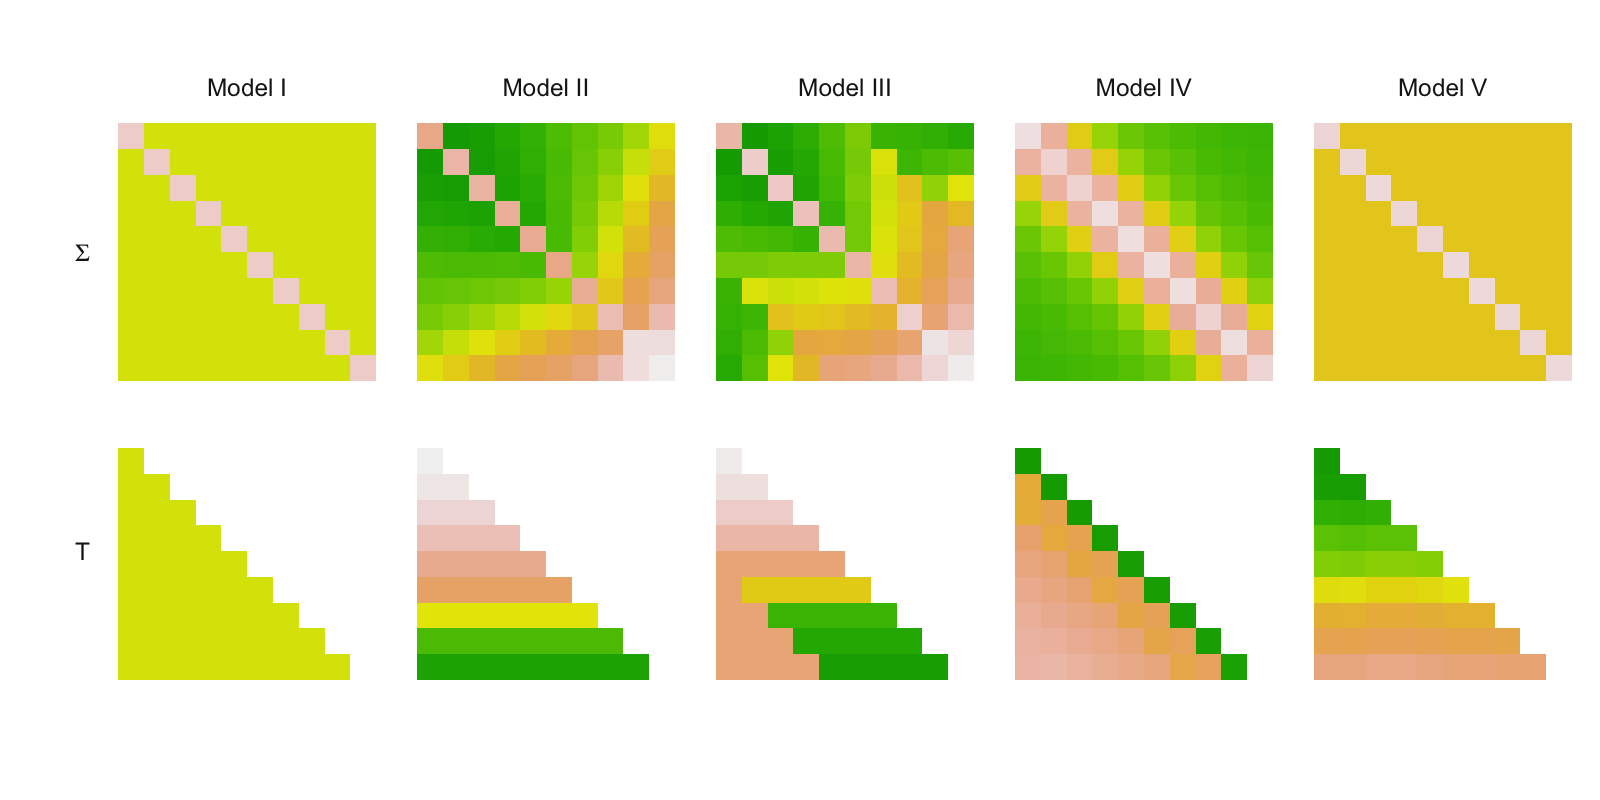
\includegraphics[width = \textwidth]{img/chapter-4/cov-cholesky-grid}%}
\caption{\textit{Heatmaps of the true covariance matrices (row 1) under simulation Models~\ref{item:cov-type-1} - Model~\ref{item:cov-type-5} and the function $\phi$ defining the corresponding Cholesky factor $T$ (row 2).} } \label{fig:true-covariance-heatmaps}
\end{center}
\end{figure}


\bigskip

%\subfile{chapter-4-subfiles/chapter-4-true-covariance-functions}

%%%%%%%%%%%%%%%%%%%%%%%%%%%%%%%%%%%%%%%%%%%%%%%%%%%%%%%%%%%%%%%%%%%%%%%%%%%%%%%%%%%%%%%%%%%%%%%%
%%%%%%%%%%%%%%%%%%%%%%%%%%%%%%%%%%%%%%%%%%%%%%%%%%%%%%%%%%%%%%%%%%%%%%%%%%%%%%%%%%%%%%%%%%%%%%%%
%%%%%%%%%%%%%%%%%%%%%%%%%%%%%%%%%%%%%%%%%%%%%%%%%%%%%%%%%%%%%%%%%%%%%%%%%%%%%%%%%%%%%%%%%%%%%%%%
%%%%%%%%%%%%%%%%%%%%%%%%%%%%%%%%%%%%%%%%%%%%%%%%%%%%%%%%%%%%%%%%%%%%%%%%%%%%%%%%%%%%%%%%%%%%%%%%
%%%%%%%%%%%%%%%%%%%%%%%%%%%%%%%%%%%%%%%%%%%%%%%%%%%%%%%%%%%%%%%%%%%%%%%%%%%%%%%%%%%%%%%%%%%%%%%%

\subsection{Loss functions and corresponding risk measures}
Let $\hat{\Sigma}$ be an estimator of the true $M \times M$ covariance matrix $\Sigma$. To assess performance of an estimator $\hat{\Sigma}$, we consider two commonly loss functions:
\begin{equation} \label{eq:quad-loss}
\Delta_1\left(\Sigma,\hat{\Sigma} \right) = tr\left(\left( \Sigma^{-1} \hat{\Sigma} - \mathrm{I}\right)^2 \right),
\end{equation}
\noindent
\begin{equation} \label{eq:entropy-loss}
\Delta_2\left(\Sigma,\hat{\Sigma}\right) = tr\left( \Sigma^{-1} \hat{\Sigma} \right) - log \vert \Sigma^{-1} \hat{\Sigma} \vert - M.
\end{equation}
\noindent
$\Sigma$ denotes the true covariance matrix and $\hat{\Sigma}$ is an $M \times M$ positive definite matrix. Each of these loss functions is $0$ when $\hat{\Sigma} = \Sigma$ and is positive when $\hat{\Sigma} \ne \Sigma$. Both measures of loss are scale invariant. If we let random vector $Y$ have covariance matrix $\Sigma$, and define the $Z$ as some linear transformation of $Y$:

\[
Z = CY. 
\]
\noindent
for some $M \times M$ matrix $C$,  then $Z$ has covariance matrix $\Sigma_Z = C \Sigma C'$. Given an estimator $\hat{\Sigma}$ of $\Sigma$, one immediately obtains an estimator for $\Sigma_Z$, $\hat{\Sigma}_Z = C \hat{\Sigma} C'$. If $C$ is invertible, then the loss functions $\Delta_1$ and $\Delta_2$ satisfy
\[
\Delta_i\left(\Sigma,\hat{\Sigma}\right) = \Delta_i\left(C \Sigma C', C \hat{\Sigma}C' \right). 
\]
\noindent
The first loss $\Delta_1$, or the quadratic loss, measures the discrepancy between $\left(\Sigma^{-1} \hat{\Sigma}\right)$ and the identity matrix with the squared Frobenius norm. The Frobenius norm of a matrix $A$ is given by 

\[
\vert \vert A \vert \vert_F^2 = \mbox{tr}\left(A A'\right).
\]
\noindent
The second loss $\Delta_2$ is commonly referred to as the entropy loss; it gives the Kullback-Leibler divergence of two multivariate Normal densities with the same mean and the two corresponding covariance matrices. The quadratic loss penalizes overestimates more than underestimates, so ``smaller'' estimates are favored more under $\Delta_1$ than $\Delta_2$. For example, among the class of estimators comprised of scalar multiples $cS$ of the sample covariance matrix, \cite{haff1980empirical} established that $S$ is optimal under $\Delta_2$, while the smaller estimator $\frac{NS}{N+M+1}$ is optimal under $\Delta_1$. 

\bigskip

Given $\Sigma$, the corresponding values of the risk functions are obtained by taking expectations:

\begin{equation*}
R_i \left(\Sigma,\hat{\Sigma}\right) = E_\Sigma\left[\Delta_i\left(\Sigma,\hat{\Sigma}\right)\right], \quad i = 1,2.
\end{equation*}
\noindent
We prefer an estimator $\hat{\Sigma}$ with smaller risk.  Given $\Sigma$, we can estimate the risk of an estimator via Monte Carlo approximation. 

%%%%%%%%%%%%%%%%%%%%%%%%%%%%%%%%%%%%%%%%%%%%%%%%%%%%%%%%%%%%%%%%%%%%%%%%%%%%%%%%%%%%%%%%%%%%%%%%
%%%%%%%%%%%%%%%%%%%%%%%%%%%%%%%%%%%%%%%%%%%%%%%%%%%%%%%%%%%%%%%%%%%%%%%%%%%%%%%%%%%%%%%%%%%%%%%%
%%%%%%%%%%%%%%%%%%%%%%%%%%%%%%%%%%%%%%%%%%%%%%%%%%%%%%%%%%%%%%%%%%%%%%%%%%%%%%%%%%%%%%%%%%%%%%%%
%%%%%%%%%%%%%%%%%%%%%%%%%%%%%%%%%%%%%%%%%%%%%%%%%%%%%%%%%%%%%%%%%%%%%%%%%%%%%%%%%%%%%%%%%%%%%%%%
%%%%%%%%%%%%%%%%%%%%%%%%%%%%%%%%%%%%%%%%%%%%%%%%%%%%%%%%%%%%%%%%%%%%%%%%%%%%%%%%%%%%%%%%%%%%%%%%

\subsubsection{Alternative estimators}
%\subfile{chapter-4-subfiles/chapter-4-benchmark-estimators}
The following estimators serve as benchmarks for performance under the five simulation settings outlined above: the MCD polynomial estimator $\hat{\Sigma}_{poly}$, the sample covariance matrix $S$, the soft thresholding estimator $S^\lambda$, and the tapering estimator $S^\omega$. We will review the general definitions of these, but for detailed discussion of the construction and properties of these estimators, see Sections~\ref{elementwise-shrinkage-estimators} and \ref{chapter-1-matrix-decompositions}.

\bigskip

{\needsparaphrased{TO DO: descriptions of the oracle estimators}}

\bigskip

In the spirit of the GLM, the MCD polynomial estimator is a particular case of estimators which model the components of the Cholesky decomposition using covariates. The polynomial estimator takes the GARPs and IVs to be polynomials of lag and time, respectively:

\begin{align*}
\begin{split}  \label{eq:GARP-IV-parametric-model}
\phi_{jk} &= z'_{jk} \gamma \\
\log \sigma^2_{j} &= z'_{j}\lambda, 
\end{split}
\end{align*}
\noindent
for $j = 1,\dots, M$, $k = 1,\dots, j-1$. The vectors $z_j$ and $z_{jk}$ are of dimension $q \times 1$ and $p \times 1$  which hold covariates

\begin{align}
\begin{split} 
z'_{jk} &= \left(1, t_j - t_k, \left(t_j - t_k\right)^2,\dots, \left(t_j - t_k\right)^{p-1}\right)', \\
z'_{j}  &= \left(1, t_j, \dots, t_j^{q-1}\right)'.
\end{split}
\end{align} \label{eq:mcd-polynomial-model}
\noindent
where the orders of the polynomials, $p$ and $q$, are chosen by BIC. 

\bigskip

\cite{rothman2009generalized} presented a class of generalized thresholding estimators, including the soft-thresholding estimator given by

\[
S^{\lambda}=   \begin{bmatrix} \mbox{sign}\left(s_{ij}\right) \left(s_{ij} - \lambda\right)_+ \end{bmatrix},
\]
\noindent 
where $\sigma^*_{ij}$ denotes the $i$-$j^{th}$ entry of the sample covariance matrix, and $\lambda$ is a penalty parameter controlling the amount of shrinkage applied to the empirical estimator. 

\bigskip

The tapering estimator proposed by \cite{cai2010optimal} is given by
\[
S^{\omega} =  \begin{bmatrix} \omega_{ij}^k s_{ij} \end{bmatrix},
\]
\noindent
where the $\omega_{ij}^k$ are given by 
\begin{equation*}
\omega^k_{ij} = k_h^{-1} \left[ \left( k - \vert i-j\vert\right)_+ - \left(k_h - \vert i-j\vert\right)_+ \right],
\end{equation*}
\noindent
The weights $\omega^k_{ij}$ are controlled by a tuning parameter, $k$,  which can take integer values between 0 and $M$. Without loss of generality,  we assume that $k_h = k/2$ is even. The weights may be rewritten as
\begin{align*}
\omega_{ij} = \left\{\begin{array}{ll} 1, & \vert i -j \vert \le k_h \\
                             2 - \frac{i - j}{k_h}, & k_h < \vert  i -j \vert \le k, \\
                             0, & \mbox{otherwise}  \end{array} \right.
\end{align*}
\noindent

\bigskip

Tuning parameter selection for the regularized versions of the sample covariance matrix was performed using cross validation. Under certain conditions pertaining to the ratio of sample sizes of the training and validation datasets, the $K$-fold cross validation criterion is a consistent estimator of the Frobenius norm risk. It is defined 

\begin{equation} \label{eq:K-fold-matrix--cv}
\mbox{CV}_F\left(\lambda \right) = \argmin{\lambda} K^{-1} \sum_{k = 1}^K  \vert \vert\hat{\Sigma}^{\left(-k\right)} - \tilde{\Sigma}^{\left(k\right)}  \vert \vert_F^2, 
\end{equation}
\noindent
There is little established about the optimal method for tuning parameter selection in for the class of estimators based on element-wise shrinkage of the sample covariance matrix.  However, based on the results of an extensive simulation study presented in \cite{fang2016tuning}, we use $K = 10$-fold cross validation to select the tuning parameters for both the tapering estimator $S^\omega$ and the soft thresholding estimator $S^{\lambda}$. They authors implement cross validation for a number of element-wise shrinkage estimators for covariance matrices in the \cite{CVTuningCov} R package, which was used to calculate the risk estimates for $S^{\omega}$ and $S^{\lambda}$. 

\bigskip

As discussed in Chapter 1, in the limit, soft thresholding produces a positive definite estimator with probability tending to 1 (\cite{rothman2009generalized}), however element-wise shrinkage estimators of the covariance matrix, including the soft thresholding estimator, are not guaranteed to be positive definite. We observed simulations runs which yielded a soft thresholding estimator that was indeed not positive definite.  In this case, the estimate has at least one eigenvalue less than or equal to zero, and the evaluation of the entropy loss \ref{eq:entropy-loss} is undefined. To enable the evaluation of the entropy loss, we coerced these estimates to the ``nearest'' positive definite estimate via application of the technique presented in \cite{cheng1998modified}.  For a symmetric matrix $A$, which is not positive definite,  a modified Cholesky algorithm produces a symmetric perturbation matrix $E$ such that $A + E$ is positive definite.

\bigskip

\cite{pan2003modelling} present an iterative procedure for estimating coefficient vectors $\lambda$, $\gamma$ of the polynomial model \ref{eq:mcd-polynomial-model}. Their algorithm uses a quasi-Newton step for computing the MLE under the multivariate normal likelihood. Their work is  is implemented in the JMCM package for \textsf{R}, which we used to compute the polynomial MCD estimates.  For implementation details, see \cite{pan2017jmcm}. 	 


%\subfile{chapter-4-subfiles/chapter-4-benchmark-study-discussion}

%%%%%%%%%%%%%%%%%%%%%%%%%%%%%%%%%%%%%%%%%%%%%%%%%%%%%%%%%%%%%%%%%%%%%%%%%%%%%%%%%%%%%%%%%%%%%%%%
%%%%%%%%%%%%%%%%%%%%%%%%%%%%%%%%%%%%%%%%%%%%%%%%%%%%%%%%%%%%%%%%%%%%%%%%%%%%%%%%%%%%%%%%%%%%%%%%
%%%%%%%%%%%%%%%%%%%%%%%%%%%%%%%%%%%%%%%%%%%%%%%%%%%%%%%%%%%%%%%%%%%%%%%%%%%%%%%%%%%%%%%%%%%%%%%%
%%%%%%%%%%%%%%%%%%%%%%%%%%%%%%%%%%%%%%%%%%%%%%%%%%%%%%%%%%%%%%%%%%%%%%%%%%%%%%%%%%%%%%%%%%%%%%%%
%%%%%%%%%%%%%%%%%%%%%%%%%%%%%%%%%%%%%%%%%%%%%%%%%%%%%%%%%%%%%%%%%%%%%%%%%%%%%%%%%%%%%%%%%%%%%%%%
For each of the covariance models, we generated a set of observations of sample size $N = 50, 100$ from a multivariate normal distribution for each of three different values of within-subject sample size $M = 10, 20, 30$. To generate data according to Models II and III, which are parameterized in terms of the components of the Cholesky decomposition, the Cholesky factor $T$ and diagonal innovation variance matrix $D$ are constructed by evaluating $\phi$ and $\sigma^2$ at the fixed observation times. The data are then sampled according to the multivariate normal distribution with covariance matrix $\Sigma = T^{-1} D {T'}^{-1}$. Given covariance matrix $\Sigma$, risk estimates are obtained from$N_{sim} = 100$ samples from an $M$-dimensional multivariate Normal distribution with mean zero and the same covariance.  Since construction of the sample covariance matrix $S$, $S^\omega$, and $S^\lambda$ rely on having an equal number of regularly-spaced observations on each subject, simulations comparing performance across estimators were conducted using complete data with common measurement times across all $N$ subjects. 

\bigskip

Our second concern in evaluation of our methods is how performance changes when the data exhibit varying degrees of sparsity. We fix the number of sampled trajectories $N$ and vary $M$, the size of the set  of possible measurement times

\[
t_1,\dots, t_M.
\]
\noindent
We generate irregular data by first generating a complete dataset 

\begin{align*}
Y_1 &= \left(y_1\left(t_1\right), y_1\left(t_2\right), \dots, y_1\left(t_M\right)\right)' \\
Y_2 &= \left(y_2\left(t_1\right), y_2\left(t_2\right), \dots, y_2\left(t_M\right)\right)' \\
&\vdots \\
Y_N &= \left(y_N\left(t_1\right), y_N\left(t_2\right), \dots, y_N\left(t_M\right)\right)',
\end{align*}
\noindent
where $Y_1,\dots, Y_N$ are independently and identically distributed according to an $M$-dimensional multivariate Normal distribution with mean zero and having covariance structure identical to one of Models I - V in \ref{table:simulation-model-list}. To induce sparsity, we subsample from the complete data $\left\{y_i\left(t_j\right) \right\}$, $i = 1,\dots, N$, $j = 1,\dots, M$, randomly omitting an observation $y_i\left(t_j\right)$ with probability $0.05$, $0.07$, and $0.09$. For both sets of simulations, the smoothing parameters for the smoothing spline and P-spline estimators were selected using both leave-one-subject-out cross validation $\mbox{losoCV}\left(\lambda\right)$ and unbiased risk estimate $\mbox{U}\left(\lambda\right)$. Given the selected values of the tuning parameters, we computed the estimated covariance matrix and compared it to the true covariance matrix via entropy loss and quadratic loss. 


%%%%%%%%%%%%%%%%%%%%%%%%%%%%%%%%%%%%%%%%%%%%%%%%%%%%%%%%%%%%%%%%%%%%%%%%%%%%%%%%%%%%%%%%%%%%%%%%
%%%%%%%%%%%%%%%%%%%%%%%%%%%%%%%%%%%%%%%%%%%%%%%%%%%%%%%%%%%%%%%%%%%%%%%%%%%%%%%%%%%%%%%%%%%%%%%%
%%%%%%%%%%%%%%%%%%%%%%%%%%%%%%%%%%%%%%%%%%%%%%%%%%%%%%%%%%%%%%%%%%%%%%%%%%%%%%%%%%%%%%%%%%%%%%%%
%%%%%%%%%%%%%%%%%%%%%%%%%%%%%%%%%%%%%%%%%%%%%%%%%%%%%%%%%%%%%%%%%%%%%%%%%%%%%%%%%%%%%%%%%%%%%%%%
%%%%%%%%%%%%%%%%%%%%%%%%%%%%%%%%%%%%%%%%%%%%%%%%%%%%%%%%%%%%%%%%%%%%%%%%%%%%%%%%%%%%%%%%%%%%%%%%


\section{Results}

\subsection{Simulations with complete data}
Figure~\ref{fig:cov-estimate-lattice} provides a visual summary of the qualitative differences between the estimates resulting from each of the eight methods of estimation for the five covariance structures used for simulation. The first row in the grid shows the surface plot of each of the true covariance structures, and each row thereafter corresponds to the five covariance estimates for the given estimation method. The surface plots of the oracle estimate in the second row serve as a point of reference for the `gold standard` in each scenario, since the oracle estimates were constructed assuming that the functional form of the covariance is known (either the full covariance structure or the components of the Cholesky decomposition.) The corresponding estimates of the Cholesky factor $T$ for the estimators based on the modified Cholesky decomposition are shown in Figure~\ref{fig:chol-estimate-lattice}, and the decomposition of the $\hat{T}$ corresponding to the smoothing spline ANOVA estimator $\hat{\Sigma}_{SS}$ into functional components is displayed in Figure~\ref{fig:ssanova-component-lattice}

%\subfile{chapter-4-subfiles/chapter-4-cov-lattice-ggplot}

\begin{figure}[H] 
\centering
\caption{\textit{Covariance Model~\ref{item:cov-type-1} - Model~\ref{item:cov-type-5} used for simulation and corresponding estimates. The columns in the grid correspond to each simulation model. The first row of shows the true covariance structure, and each row beneath corresponds to each of the estimators.}}
  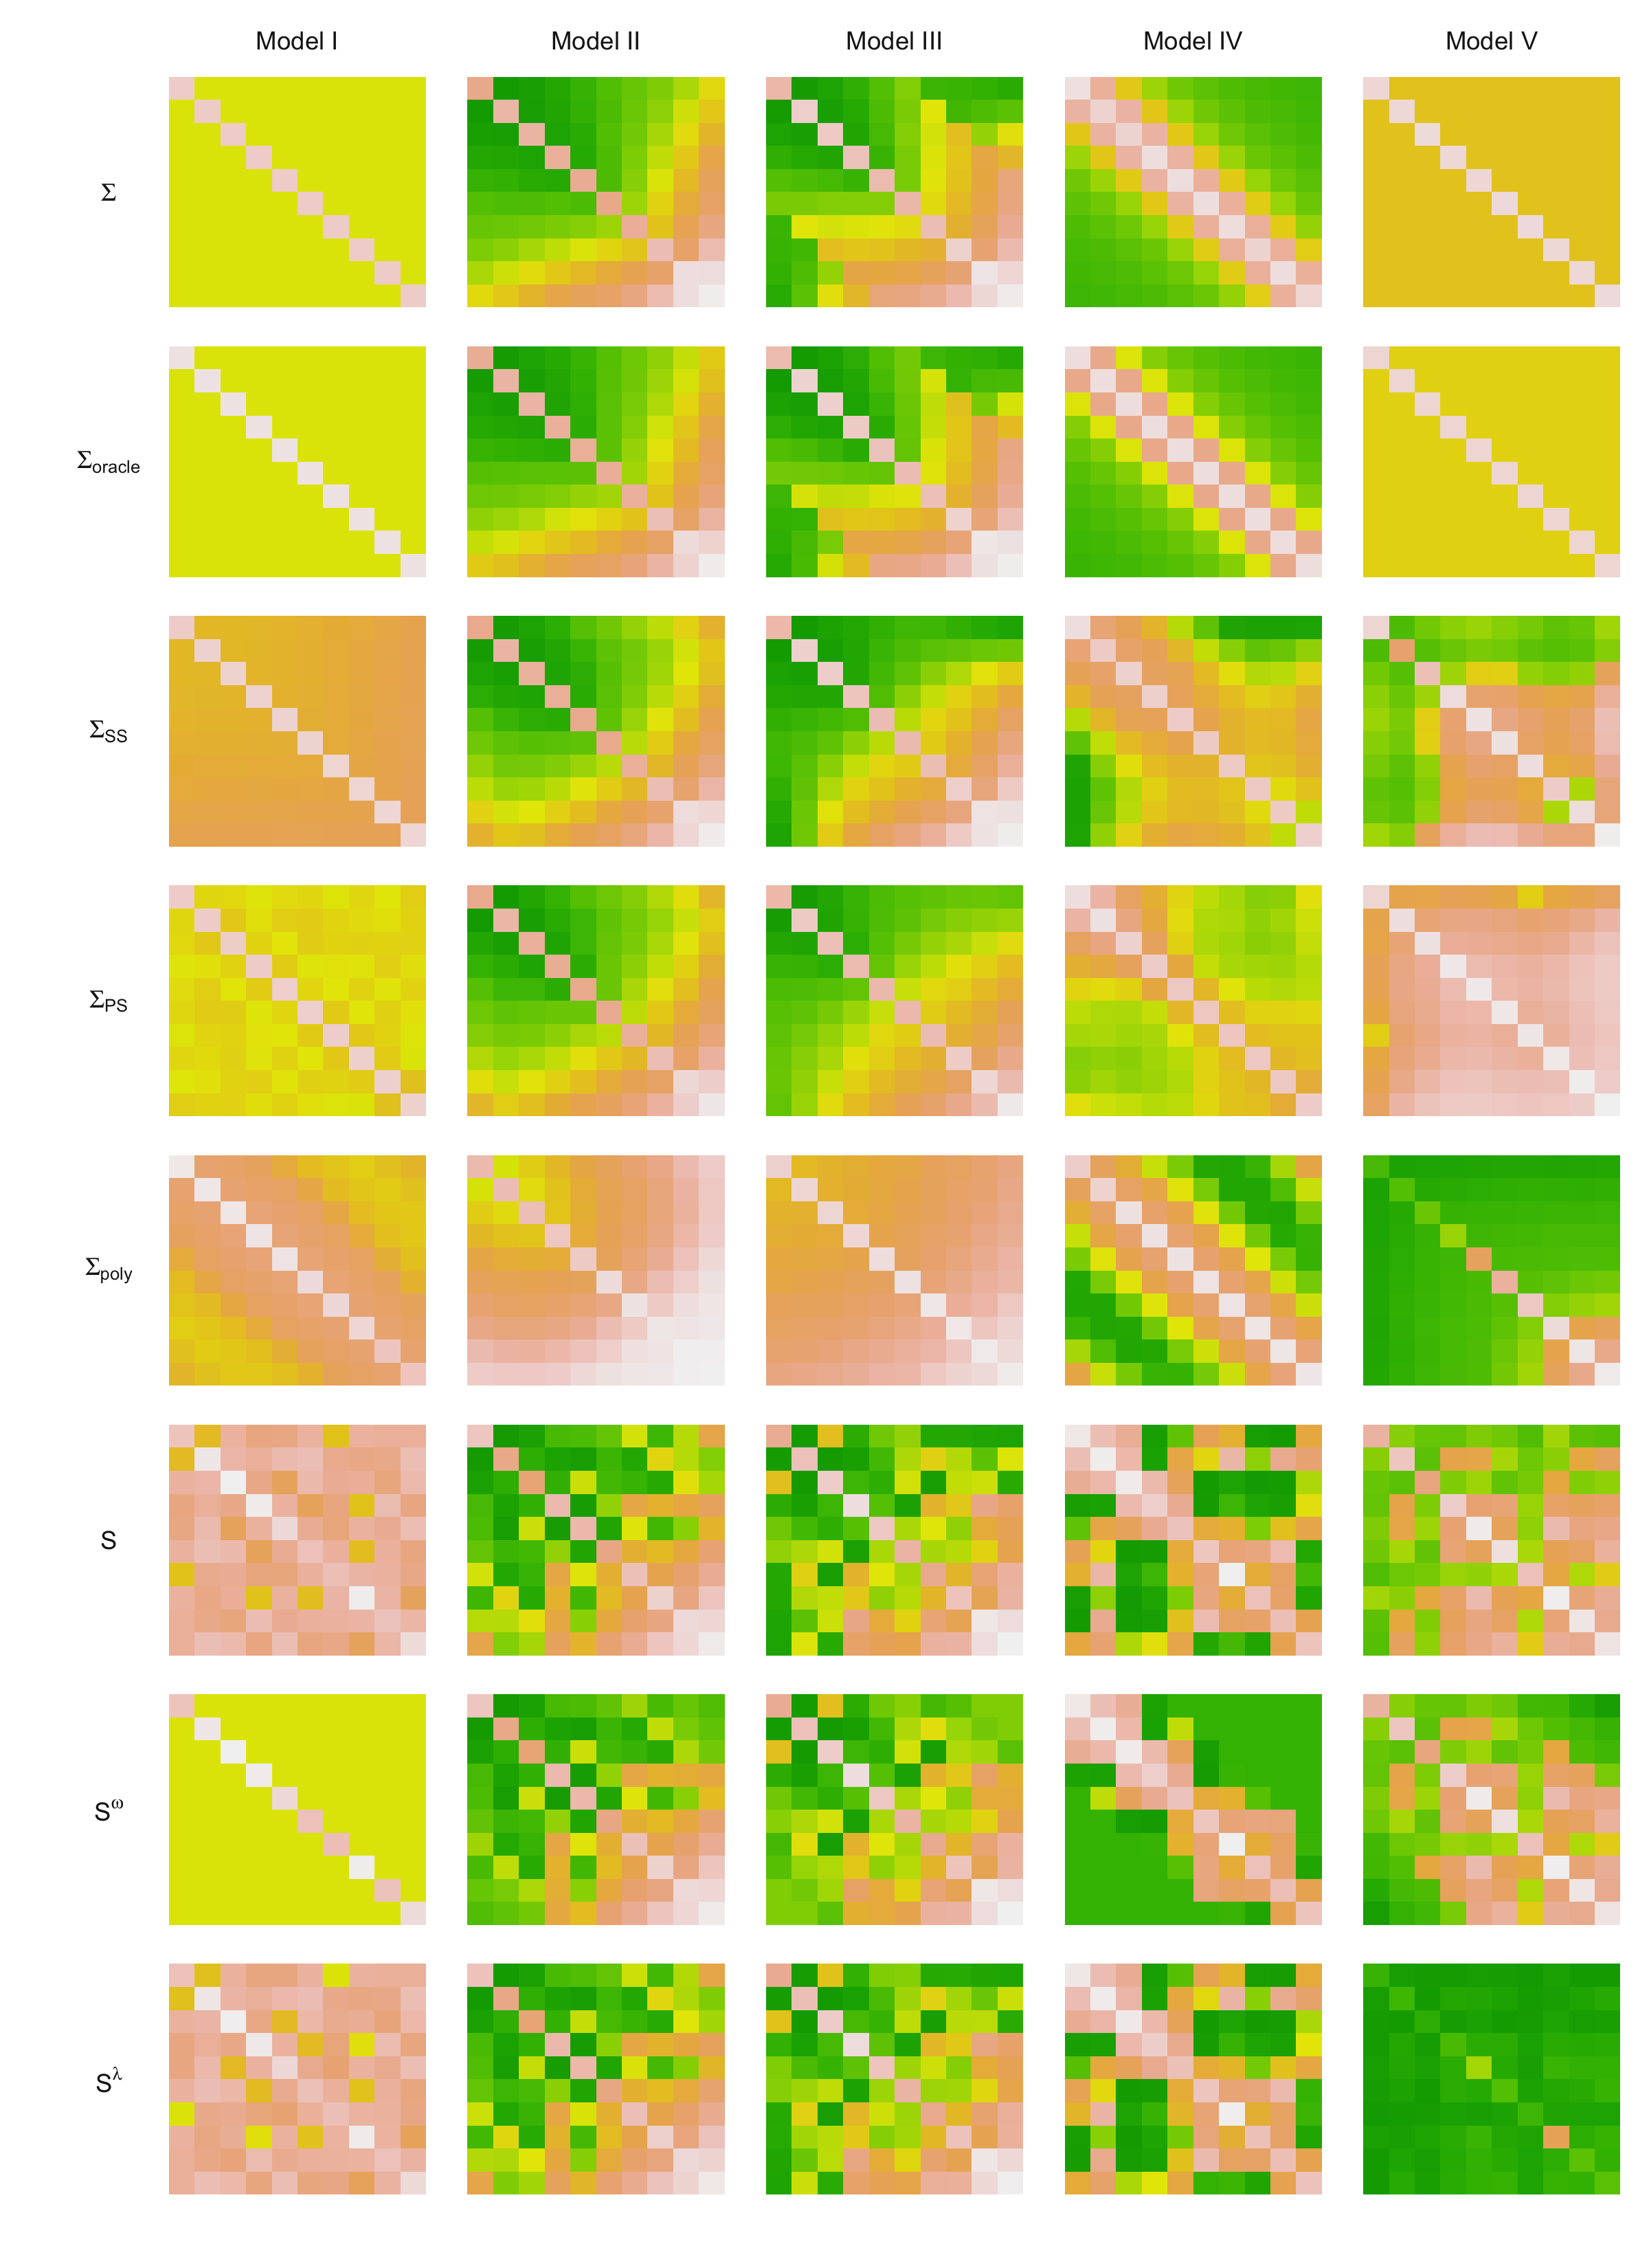
\includegraphics[width = 1\textwidth]{img/chapter-4/cov-estimate-lattice}\label{fig:cov-estimate-lattice}
\end{figure}

\begin{figure}[H] 
\centering
\caption{\textit{The generalized autoregressive coefficient function $\phi$ which defines the elements of the true lower triangle of Cholesky factor $T$ corresponding to Model~\ref{item:cov-type-1} - Model~\ref{item:cov-type-5} and estimates of the same surface for estimators based on the modified Cholesky decomposition. The true covariance structure is displayed across the top row.}}
  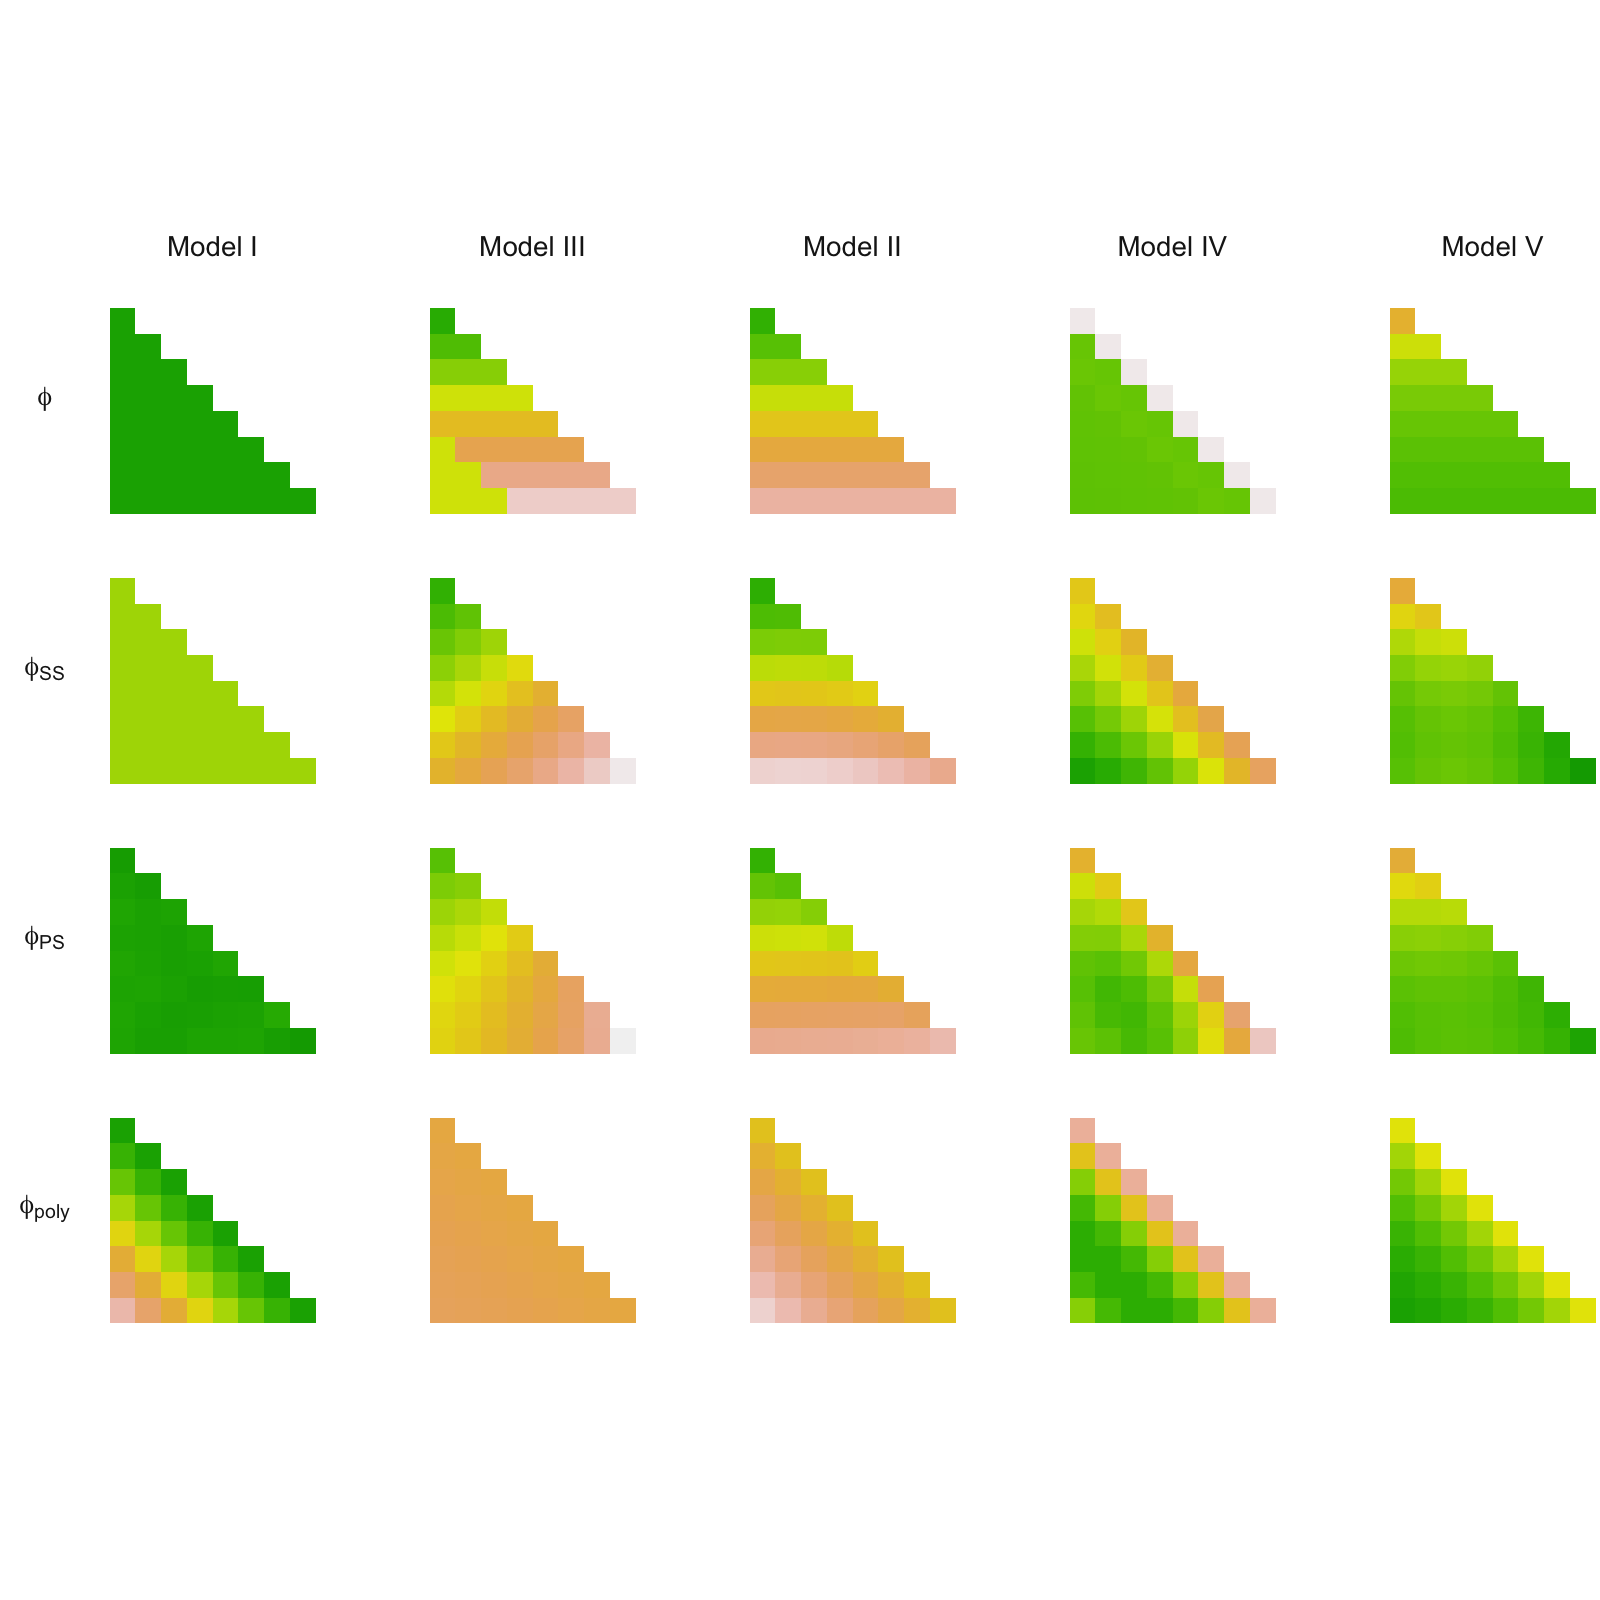
\includegraphics[width = 1\textwidth]{img/chapter-4/cholesky-estimate-lattice}
  \label{fig:chol-estimate-lattice}
\end{figure}

%\subfile{chapter-4-subfiles/chapter-4-ssanova-lattice-ggplot}

\begin{figure}[H] 
\caption{\textit{Estimated functional components of the smoothing spline ANOVA decomposition $\phi = \phi_1 + \phi_2 + \phi_{12}$ for $\hat{\Sigma}_{SS}$ under each simulation model I - V.}}
  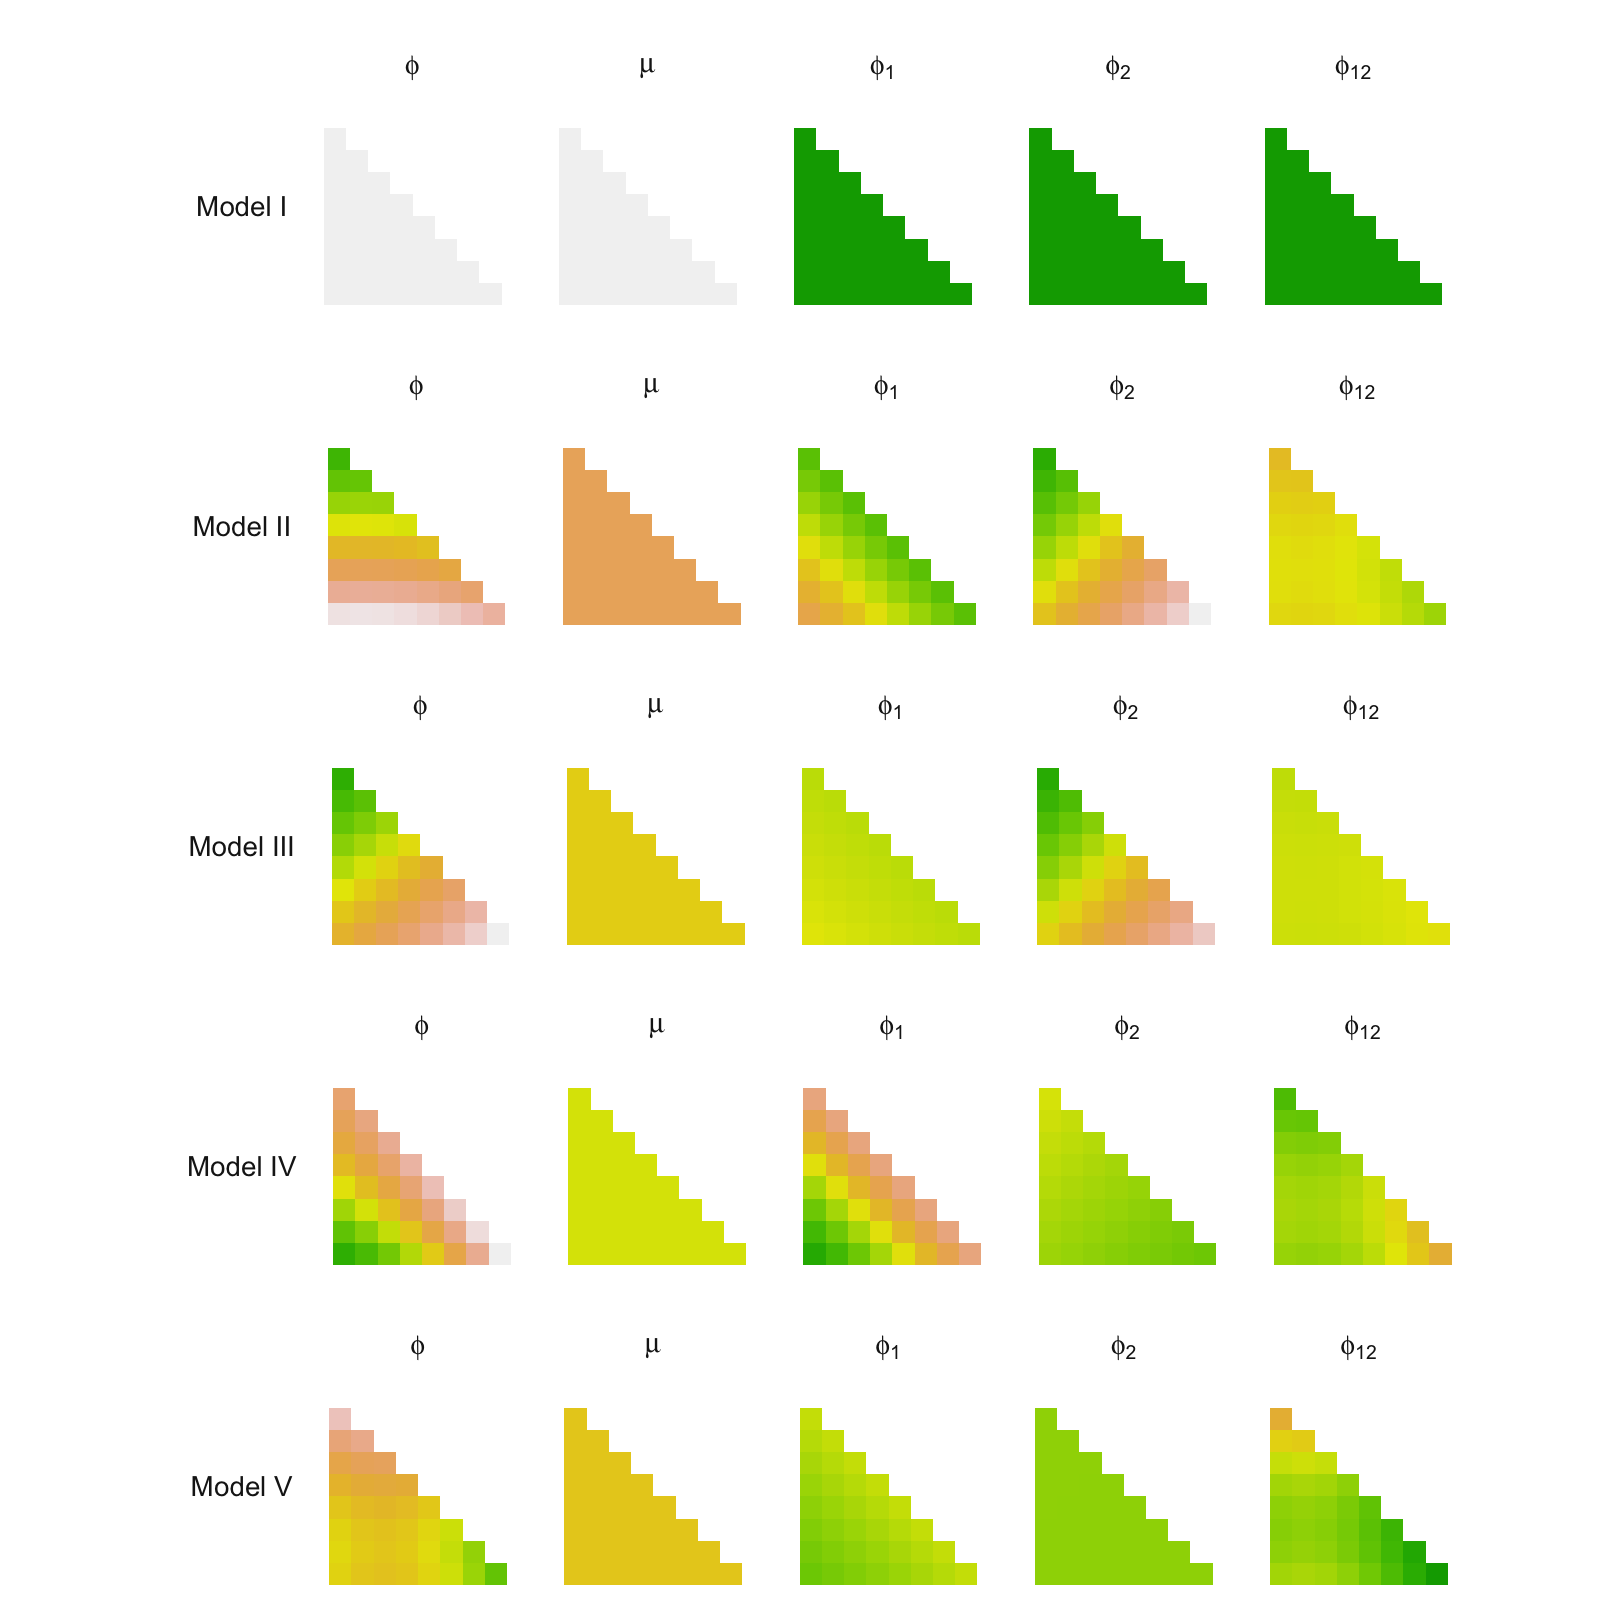
\includegraphics[width = \textwidth]{img/chapter-4/ssanova-estimate-lattice} \label{fig:ssanova-component-lattice}
\end{figure}

\bigskip
The results of the simulations for complete data under entropy loss are presented in Tables~\ref{table:simulation-1-entropy-loss-sigma-1} - \ref{table:simulation-1-entropy-loss-sigma-5}. Risk estimates under quadratic loss, while there is not agreement between results every time, qualitatively, they are similar in nature to those with entropy loss. These are left to the Appendix, Tables~\ref{table:simulation-1-quad-loss-sigma-1}-\ref{table:simulation-1-quad-loss-sigma-5}. Since both loss functions are not standardized, they cannot be compared across dimensions $M$.

\bigskip

In general, our estimators outperform the alternative estimators across the five covariance structures. This is not surprising; the soft thresholding estimator assumes no ordering of the variables of the random vector, which all but one of the generating structures exhibit. The tapering estimator assumes that the absolute value of the covariance decays as $l$ increases; only model IV satisfies this. The parametric estimator based on the modified Cholesky decomposition assumes that $\phi$ can be modeled as a univariate function of $l$, which does not hold for any of the models, save model IV.

\bigskip

The smoothing spline estimator outperforms the P-spline estimator in cases where the underlying covariance structure cannot be modeled as a multiplicative function of $l$ and $m$ - namely, model II. The P-spline estimator outperforms the smoothing spline estimator under model IV, likely due to the advantage of trivially change the order of the difference penalty. When the difference order is specified so that the generating model belongs to the null space $\hilbert_0$, the search for the optimal set of smoothing parameters is a much easier task.   
 
\bigskip
%%%%%%%%%%%%%%%%%%%%%%%%%%%%%%%%%%%%%%%%%%%%%%%%%%%%%%%%%%%%%%%%%%%%%%%%%%%%%%%%%%%%%%%%%%%%%%%%
%%%%%%%%%%%%%%%%%%%%%%%%%%%%%%%%%%%%%%%%%%%%%%%%%%%%%%%%%%%%%%%%%%%%%%%%%%%%%%%%%%%%%%%%%%%%%%%%
\setlength{\dashlinedash}{0.5pt}
\setlength{\dashlinegap}{1pt}
\setlength{\arrayrulewidth}{0.2pt}
%\subfile{chapter-4-subfiles/simulation-study-1-entropy-table-model-1}
% latex table generated in R 3.4.3 by xtable 1.8-2 package
% Tue Mar  6 10:27:03 2018
\begin{table}[H]
\centering
\caption{\textit{Multivariate normal simulations for Model I. Estimated entropy risk is reported for our smoothing spline ANOVA estimator and P-spline estimator, the oracle estimator for each covariance structure, the parametric polynomial estimator of Pan and MacKenzie (2003), the sample covariance matrix, the tapered sample covariance matrix, and the soft thresholding estimator.}}
\begin{tabular}{lrrrrrrrr}
 & $M$ &$\hat{\Sigma}_{SS}$& $\hat{\Sigma}_{PS}$ &$\hat{\Sigma}_{oracle}$& $\hat{\Sigma}_{poly}$ & $S$ &$S^\omega$& $S^\lambda$ \\ 
  \hline
$N = 50$ & 10 & 0.0749 & 0.1261 & 0.0135 & 0.1102 & 1.2047 & 0.5369 & 1.1742 \\ 
   & $20$ & 0.0872 & 0.1713 & 0.0229 & 0.1096 & 4.9850 & 1.3957 & 4.7796 \\ 
   & $30$ & 0.1102 & 0.1969 & 0.0196 & 0.1127 & 12.5517 & 2.8019 & 11.3175 \\ 
 $N = 100$ & $10$ & 0.0451 & 0.0671 & 0.0105 & 0.0531 & 0.5685 & 0.2045 & 0.5236 \\ 
   & $20$ & 0.0425 & 0.0965 & 0.0105 & 0.0512 & 2.2831 & 0.5724 & 2.1358 \\ 
   & $30$ & 0.0431 & 0.1148 & 0.0139 & 0.0472 & 5.2770 & 1.2430 & 4.9126 \\ 
   \hline
\end{tabular}
\label{table:simulation-1-entropy-loss-sigma-1}
\end{table}


%%%%%%%%%%%%%%%%%%%%%%%%%%%%%%%%%%%%%%%%%%%%%%%%%%%%%%%%%%%%%%%%%%%%%%%%%%%%%%%%%%%%%%%%%%%%%%%%
%%%%%%%%%%%%%%%%%%%%%%%%%%%%%%%%%%%%%%%%%%%%%%%%%%%%%%%%%%%%%%%%%%%%%%%%%%%%%%%%%%%%%%%%%%%%%%%%
% latex table generated in R 3.4.3 by xtable 1.8-2 package
% Tue Mar  6 10:27:30 2018

\begin{table}[H]
\centering
\caption{\textit{Multivariate normal simulations for model II.}}
\begin{tabular}{lrrrrrrrr}
 & $M$ &$\hat{\Sigma}_{SS}$& $\hat{\Sigma}_{PS}$ &$\hat{\Sigma}_{oracle}$& $\hat{\Sigma}_{poly}$ & $S$ &$S^\omega$& $S^\lambda$ \\ 
  \hline
   $N = 50$ & $10$ & 0.0899 & 0.3423 & 0.0581 & 4.7673 & 1.2832 & 1.4644 & 1.1770 \\ 
   & $20$ & 0.0949 & 1.3640 & 0.0439 & 97.2334 & 5.1665 & 21.6407 & 39.3522 \\ 
     & $30$ & 0.0811 & 2.6485 & 0.0627 & 1539.6646 & 12.3582 & 55.3674 & 133.9980 \\ 
  $N = 100$ & 10 & 0.0457 & 0.2945 & 0.0386 & 4.7911 & 0.5812 & 0.8335 & 0.5628 \\ 
    & $20$ & 0.0416 & 1.2875 & 0.0269 & 98.1989 & 2.3364 & 10.1841 & 10.0864 \\ 
    & $30$ & 0.0367 & 2.4365 & 0.0288 & 1582.4795 & 5.2389 & 33.5207 & 62.5030 \\ 
   \hline
\end{tabular}
\label{table:simulation-1-entropy-loss-sigma-2}
\end{table}


%%%%%%%%%%%%%%%%%%%%%%%%%%%%%%%%%%%%%%%%%%%%%%%%%%%%%%%%%%%%%%%%%%%%%%%%%%%%%%%%%%%%%%%%%%%%%%%%
%%%%%%%%%%%%%%%%%%%%%%%%%%%%%%%%%%%%%%%%%%%%%%%%%%%%%%%%%%%%%%%%%%%%%%%%%%%%%%%%%%%%%%%%%%%%%%%%
%\subfile{chapter-4-subfiles/simulation-study-1-entropy-table-model-2}
%\subfile{chapter-4-subfiles/simulation-study-1-entropy-table-model-3}
% latex table generated in R 3.4.3 by xtable 1.8-2 package
% Tue Mar  6 10:27:35 2018


\begin{table}[H]
\centering
\caption{\textit{Multivariate normal simulations for model III.} }
\begin{tabular}{lrrrrrrrr}
 & $M$ &$\hat{\Sigma}_{SS}$& $\hat{\Sigma}_{PS}$ &$\hat{\Sigma}_{oracle}$& $\hat{\Sigma}_{poly}$ & $S$ &$S^\omega$& $S^\lambda$ \\ 
   \hline
 $N = 50$ & 10 & 0.3416 & 0.1065 & 0.0619 & 3.0108 & 1.2030 & 1.1460 & 1.1467 \\ 
      & $20$ & 1.1140 & 0.2555 & 0.0695 & 62.7522 & 4.9824 & 17.2244 & 14.9189 \\ 
    & $30$ & 2.3215 & 0.6242 & 0.0576 & 1091.1933 & 12.4792 & 49.9135 & 121.7795 \\ 
     $N = 100$ & $10$ & 0.2904 & 0.0579 & 0.0268 & 3.0383 & 0.5699 & 0.5545 & 0.5371 \\ 
     & $20$ & 1.1963 & 0.2011 & 0.0275 & 62.8960 & 2.2700 & 11.8274 & 9.5217 \\ 
    & $30$ & 2.2811 & 0.3845 & 0.0221 & 1105.0449 & 5.2234 & 29.1693 & 60.3529 \\ 
   \hline
\end{tabular}
\label{table:simulation-1-entropy-loss-sigma-3}
\end{table}

%%%%%%%%%%%%%%%%%%%%%%%%%%%%%%%%%%%%%%%%%%%%%%%%%%%%%%%%%%%%%%%%%%%%%%%%%%%%%%%%%%%%%%%%%%%%%%%%
%%%%%%%%%%%%%%%%%%%%%%%%%%%%%%%%%%%%%%%%%%%%%%%%%%%%%%%%%%%%%%%%%%%%%%%%%%%%%%%%%%%%%%%%%%%%%%%%
%\subfile{chapter-4-subfiles/simulation-study-1-entropy-table-model-4}
% latex table generated in R 3.4.3 by xtable 1.8-2 package
% Tue Mar  6 10:27:39 2018
\begin{table}[H]
\centering
\caption{\textit{Multivariate normal simulations for model IV.}}
\begin{tabular}{lrrrrrrrr}
 & $M$ &$\hat{\Sigma}_{SS}$& $\hat{\Sigma}_{PS}$ &$\hat{\Sigma}_{oracle}$& $\hat{\Sigma}_{poly}$ & $S$ &$S^\omega$& $S^\lambda$ \\ 
  \hline
 $N = 50$ & $10$ & 0.3422 & 0.1966 & 0.0217 & 0.7144 & 1.2218 & 0.7397 & 1.1921 \\ 
   & $20$ & 0.9208 & 0.3499 & 0.0286 & 1.4588 & 4.9091 & 1.9786 & 4.9206 \\ 
       & $30$ & 1.5992 & 0.5100 & 0.0283 & 2.2173 & 12.6114 & 3.7440 & 12.1489 \\ 
     $N = 100$ & 10 & 0.3047 & 0.2237 & 0.0125 & 0.6958 & 0.5570 & 0.3168 & 0.5515 \\ 
       & $20$ & 0.8911 & 0.3704 & 0.0105 & 1.4813 & 2.2659 & 0.9365 & 2.2474 \\ 
       & $30$ & 1.5213 & 0.5282 & 0.0134 & 2.2228 & 5.2106 & 1.9312 & 5.2111 \\ 
   \hline
\end{tabular} 
\label{table:simulation-1-entropy-loss-sigma-4}
\end{table}

%%%%%%%%%%%%%%%%%%%%%%%%%%%%%%%%%%%%%%%%%%%%%%%%%%%%%%%%%%%%%%%%%%%%%%%%%%%%%%%%%%%%%%%%%%%%%%%%
%%%%%%%%%%%%%%%%%%%%%%%%%%%%%%%%%%%%%%%%%%%%%%%%%%%%%%%%%%%%%%%%%%%%%%%%%%%%%%%%%%%%%%%%%%%%%%%%
%\subfile{chapter-4-subfiles/simulation-study-1-entropy-table-model-5}
% latex table generated in R 3.4.3 by xtable 1.8-2 package
% Tue Mar  6 10:27:42 2018
\begin{table}[H]
\centering
\caption{\textit{Multivariate normal simulations for model V.}}
\begin{tabular}{lrrrrrrrr}
 & $M$ &$\hat{\Sigma}_{SS}$& $\hat{\Sigma}_{PS}$ &$\hat{\Sigma}_{oracle}$& $\hat{\Sigma}_{poly}$ & $S$ &$S^\omega$& $S^\lambda$ \\ 
  \hline
 $N = 50$ & $10$ & 0.2743 & 0.2464 & 0.0986 & 1.2420 & 1.2023 & 18.5222 & 2.9824 \\ 
  & $20$ & 0.7526 & 0.8772 & 0.2512 & 2.8557 & 5.0195 & 34.6618 & 13.8690 \\ 
  & $30$ & 1.1776 & 0.9791 & 0.2641 & 4.5791 & 12.3460 & 46.5437 & 26.1364 \\ 
 $N = 100$ & 10 & 0.2416 & 0.1722 & 0.0520 & 1.1491 & 0.5821 & 16.4081 & 1.7397 \\ 
  & $20$ & 0.7286 & 0.2965 & 0.0827 & 2.9080 & 2.2918 & 32.5295 & 5.4649 \\ 
   & $30$ & 1.1813 & 0.4291 & 0.1799 & 4.4402 & 5.2197 & 39.2914 & 15.4295 \\ 
   \hline
\end{tabular}\label{table:simulation-1-entropy-loss-sigma-5}
\end{table}


%\subfile{chapter-4-subfiles/simulation-study-1-entropy-single-table}
%%%%%%%%%%%%%%%%%%%%%%%%%%%%%%%%%%%%%%%%%%%%%%%%%%%%%%%%%%%%%%%%%%%%%%%%%%%%%%%%%%%%%%%%%%%%%%%%
%%%%%%%%%%%%%%%%%%%%%%%%%%%%%%%%%%%%%%%%%%%%%%%%%%%%%%%%%%%%%%%%%%%%%%%%%%%%%%%%%%%%%%%%%%%%%%%%
%%%%%%%%%%%%%%%%%%%%%%%%%%%%%%%%%%%%%%%%%%%%%%%%%%%%%%%%%%%%%%%%%%%%%%%%%%%%%%%%%%%%%%%%%%%%%%%%
%%%%%%%%%%%%%%%%%%%%%%%%%%%%%%%%%%%%%%%%%%%%%%%%%%%%%%%%%%%%%%%%%%%%%%%%%%%%%%%%%%%%%%%%%%%%%%%%
%%%%%%%%%%%%%%%%%%%%%%%%%%%%%%%%%%%%%%%%%%%%%%%%%%%%%%%%%%%%%%%%%%%%%%%%%%%%%%%%%%%%%%%%%%%%%%%%
\subsection{Performance with irregularly sampled data}
%%%%%%%%%%%%%%%%%%%%%%%%%%%%%%%%%%%%%%%%%%%%%%%%%%%%%%%%%%%%%%%%%%%%%%%%%%%%%%%%%%%%%%%%%%%%%%%%
%%%%%%%%%%%%%%%%%%%%%%%%%%%%%%%%%%%%%%%%%%%%%%%%%%%%%%%%%%%%%%%%%%%%%%%%%%%%%%%%%%%%%%%%%%%%%%%%
%%%%%%%%%%%%%%%%%%%%%%%%%%%%%%%%%%%%%%%%%%%%%%%%%%%%%%%%%%%%%%%%%%%%%%%%%%%%%%%%%%%%%%%%%%%%%%%%
%%%%%%%%%%%%%%%%%%%%%%%%%%%%%%%%%%%%%%%%%%%%%%%%%%%%%%%%%%%%%%%%%%%%%%%%%%%%%%%%%%%%%%%%%%%%%%%%
%%%%%%%%%%%%%%%%%%%%%%%%%%%%%%%%%%%%%%%%%%%%%%%%%%%%%%%%%%%%%%%%%%%%%%%%%%%%%%%%%%%%%%%%%%%%%%%%
%\subfile{chapter-4-subfiles/chapter-4-missing-data-study-discussion}

Estimated risk under entropy loss is given in Tables~\ref{table:simulation-study-2-entropy-risk-model-1} - \ref{table:simulation-study-2-entropy-risk-model-5}.  Risk estimates under quadratic loss echo in sentiment and are left to the Appendix.  Performance degradation of the estimator in the presence of missing data is highly dependent on the underlying structure of the Cholesky factor of the inverse covariance matrix. For the identity matrix and for the non-truncated linear varying coefficient GARP model, we observe little change in estimated entropy risk for within subject sample sizes $M = 10$ and $M = 20$ with downsampling as compared to the estimated risk for both sample sizes in the complete data case.  Neither model selection criteria appear to perform better than the other, which suggests that when the estimated innovation variances are close to the true variances of the prediction residuals, using the unbiased risk estimate with the working residuals as substitute for the relative error is a reasonable approach to modeling. When the data are missing completely at random, the performance of the estimator remains fairly stable when 10\%, 20\%, and 30\% of the data are missing. 

%%%%%%%%%%%%%%%%%%%%%%%%%%%%%%%%%%%%%%%%%%%%%%%%%%%%%%%%%%%%%%%%%%%%%%%%%%%%%%%%%%%%%%%%%%%%%%%%
%%%%%%%%%%%%%%%%%%%%%%%%%%%%%%%%%%%%%%%%%%%%%%%%%%%%%%%%%%%%%%%%%%%%%%%%%%%%%%%%%%%%%%%%%%%%%%%%
%%%%%%%%%%%%%%%%%%%%%%%%%%%%%%%%%%%%%%%%%%%%%%%%%%%%%%%%%%%%%%%%%%%%%%%%%%%%%%%%%%%%%%%%%%%%%%%%
%%%%%%%%%%%%%%%%%%%%%%%%%%%%%%%%%%%%%%%%%%%%%%%%%%%%%%%%%%%%%%%%%%%%%%%%%%%%%%%%%%%%%%%%%%%%%%%%
%%%%%%%%%%%%%%%%%%%%%%%%%%%%%%%%%%%%%%%%%%%%%%%%%%%%%%%%%%%%%%%%%%%%%%%%%%%%%%%%%%%%%%%%%%%%%%%%
\bigskip
\setlength{\dashlinedash}{0.5pt}
\setlength{\dashlinegap}{1pt}
\setlength{\arrayrulewidth}{0.2pt}
%\subfile{chapter-4-subfiles/simulation-study-2-risk-tables-ure}
%\subfile{chapter-4-subfiles/simulation-study-2-entropy-risk-model-1}
% latex table generated in R 3.4.3 by xtable 1.8-2 package
% Fri Mar  9 20:17:59 2018
%\begin{table}[H]
%\centering
%\caption{\textit{Model 1: Entropy risk estimates and corresponding standard errors 
%                                for the MCD smoothing spline ANOVA estimator via 100 simulated multivariate
%                                normal sample of size $N = 50$
%                                when 5\%, 7\%, and 9\% of the data are missing. Risk is reported for the estimator constructed using
%                                the unbiased risk estimate and leave-one-subject-out cross validation are used for smoothing parameter selection.} }
%\label{table:simulation-study-2-entropy-risk-model-1}
%\begin{tabular}{lrrlrl}
%   $M$ & \% missing & \multicolumn{2} {c} {$\Delta_2(\hat{\Sigma}^{U}_{SS})$} & \multicolumn{2} {c} {$\Delta_2(\hat{\Sigma}^{V^*}_{SS})$}\\ \hline
%10 & 0.00 & 0.05948765 & (0.0040) & 0.07355005 & (0.0053) \\ 
%   & 0.05 & 0.07526588 & (0.0064) & 0.06118984 & (0.0044) \\ 
%   & 0.07 & 0.07013988 & (0.0047) & 0.07533206 & (0.0060) \\ 
%   \hline
% & 0.09 & 0.08318940 & (0.0056) & 0.06423959 & (0.0051) \\ 
%  15 & 0.00 & 0.08753938 & (0.0073) & 0.09178231 & (0.0073) \\ 
%   & 0.05 & 0.08081929 & (0.0052) & 0.09203281 & (0.0063) \\ 
%   \hline
% & 0.07 & 0.08584911 & (0.0091) & 0.08708120 & (0.0072) \\ 
%   & 0.09 & 0.09838363 & (0.0086) & 0.08148412 & (0.0072) \\ 
%  20 & 0.00 & 0.08742261 & (0.0077) & 0.08676581 & (0.0066) \\ 
%   \hline
% & 0.05 & 0.08524652 & (0.0069) & 0.07007607 & (0.0056) \\ 
%   & 0.07 & 0.07940546 & (0.0061) & 0.07639569 & (0.0062) \\ 
%   & 0.09 & 0.07629685 & (0.0050) & 0.08846639 & (0.0063) \\ 
%  \end{tabular}
%\end{table}

% latex table generated in R 3.4.3 by xtable 1.8-2 package
% Mon Mar 19 14:41:11 2018
\begin{table}[H]
\centering
\caption{\textit{Model 1: Risk estimates and corresponding standard errors 
                                for the MCD smoothing spline ANOVA estimator via 100 simulated multivariate
                                normal sample of size $N = 50$
                                when 10\%, 20\%, and 30\% of the data are missing. Quadratic risk 
                                $\Delta_1$ and entropy risk $\Delta_2$ are
                                reported for the estimator constructed using
                                the unbiased risk estimate for smoothing parameter selection.} }
\label{table:simulation-study-2-risk-model-1}
\begin{tabular}{lrrlrl}
   $M$ & \% missing & \multicolumn{2} {c} {$\Delta_1(\hat{\Sigma}^{U}_{SS})$}\ & \multicolumn{2} {c} {$\Delta_2(\hat{\Sigma}^{U}_{SS})$}\\ \hline
10 & 0.0 & 0.00187599 & (4e-040) & 0.0737601 & (0.0073) \\ 
   & 0.1 & 0.00266749 & (4e-040) & 0.0889576 & (0.0080) \\ 
   & 0.2 & 0.00339814 & (6e-040) & 0.1037463 & (0.0098) \\ 
   & 0.3 & 0.00662281 & (0.0011) & 0.1471518 & (0.0121) \\ 
   \hline
20 & 0.0 & 0.01846478 & (0.0153) & 0.1699198 & (0.0474) \\ 
   & 0.1 & 0.22035602 & (0.2137) & 0.3343122 & (0.1691) \\ 
   & 0.2 & 0.02071463 & (0.0074) & 0.3021184 & (0.0526) \\ 
   & 0.3 & 0.22000106 & (0.1113) & 0.5327419 & (0.1623) \\ 
  \end{tabular}
\end{table}


%%%%%%%%%%%%%%%%%%%%%%%%%%%%%%%%%%%%%%%%%%%%%%%%%%%%%%%%%%%%%%%%%%%%%%%%%%%%%%%%%%%%%%%%%%%%%%%%
%%%%%%%%%%%%%%%%%%%%%%%%%%%%%%%%%%%%%%%%%%%%%%%%%%%%%%%%%%%%%%%%%%%%%%%%%%%%%%%%%%%%%%%%%%%%%%%%
% latex table generated in R 3.4.3 by xtable 1.8-2 package
% Fri Mar  9 20:17:59 2018
%\begin{table}[H]
%\centering
%\caption{\textit{Model 2: Entropy risk estimates and corresponding standard errors.} }
%\label{table:simulation-study-2-entropy-risk-model-2}
%\begin{tabular}{lrrlrl}
%   $M$ & \% missing & \multicolumn{2} {c} {$\Delta_2(\hat{\Sigma}^{U}_{SS})$} & \multicolumn{2} {c} {$\Delta_2(\hat{\Sigma}^{V^*}_{SS})$}\\ \hline
%10 & 0.00 & 0.3476005 & (0.0080) & 0.3216708 & (0.0069) \\ 
%   & 0.05 & 0.3232649 & (0.0067) & 0.3505707 & (0.0114) \\ 
%   & 0.07 & 0.3225538 & (0.0063) & 0.3300389 & (0.0067) \\ 
%   \hline
% & 0.09 & 0.3347380 & (0.0072) & 0.3303566 & (0.0056) \\ 
%  15 & 0.00 & 0.6365878 & (0.0095) & 0.6808690 & (0.0232) \\ 
%   & 0.05 & 0.6424703 & (0.0130) & 0.6241518 & (0.0105) \\ 
%   \hline
% & 0.07 & 0.6433583 & (0.0123) & 0.6362110 & (0.0084) \\ 
%   & 0.09 & 0.6621593 & (0.0223) & 0.6396626 & (0.0145) \\ 
%  20 & 0.00 & 1.1147692 & (0.0190) & 1.1078676 & (0.0089) \\ 
%   \hline
% & 0.05 & 1.1084520 & (0.0101) & 1.1111880 & (0.0107) \\ 
%   & 0.07 & 1.1221157 & (0.0088) & 1.1406596 & (0.0117) \\ 
%   & 0.09 & 1.0973568 & (0.0093) & 1.1105763 & (0.0098) \\ 
%  \end{tabular}
%\end{table}

% latex table generated in R 3.4.3 by xtable 1.8-2 package
% Mon Mar 19 14:41:11 2018
\begin{table}[H]
\centering
\caption{\textit{Model 2: Risk estimates and corresponding standard errors.} }
\label{table:simulation-study-2-risk-model-2}
\begin{tabular}{lrrlrl}
   $M$ & \% missing & \multicolumn{2} {c} {$\Delta_1(\hat{\Sigma}^{U}_{SS})$}\ & \multicolumn{2} {c} {$\Delta_2(\hat{\Sigma}^{U}_{SS})$}\\ \hline
10 & 0.0 & 0.0525852 & (0.0108) & 0.0735172 & (0.0064) \\ 
   & 0.1 & 0.1193846 & (0.0301) & 0.1080945 & (0.0094) \\ 
   & 0.2 & 0.2625658 & (0.0464) & 0.2146169 & (0.0149) \\ 
   & 0.3 & 0.7184782 & (0.1534) & 0.3601229 & (0.0351) \\ 
   \hline
20 & 0.0 & 0.5477523 & (0.0819) & 0.0672205 & (0.0053) \\ 
   & 0.1 & 21.6916082 & (2.4816) & 0.6955444 & (0.0509) \\ 
   & 0.2 & 287.3776278 & (27.6998) & 4.2309218 & (0.2668) \\ 
   & 0.3 & 176594.9017073 & (93975.3308) & 68.9661337 & (28.3602) \\ 
  \end{tabular}
\end{table}


%%%%%%%%%%%%%%%%%%%%%%%%%%%%%%%%%%%%%%%%%%%%%%%%%%%%%%%%%%%%%%%%%%%%%%%%%%%%%%%%%%%%%%%%%%%%%%%%
%%%%%%%%%%%%%%%%%%%%%%%%%%%%%%%%%%%%%%%%%%%%%%%%%%%%%%%%%%%%%%%%%%%%%%%%%%%%%%%%%%%%%%%%%%%%%%%%
% latex table generated in R 3.4.3 by xtable 1.8-2 package
% Fri Mar  9 20:17:59 2018
%\begin{table}[H]
%\centering
%\caption{\textit{Model 3: Entropy risk estimates and corresponding standard errors.} }
%\label{table:simulation-study-2-entropy-risk-model-3}
%\begin{tabular}{lrrlrl}
%   $M$ & \% missing & \multicolumn{2} {c} {$\Delta_2(\hat{\Sigma}^{U}_{SS})$} & \multicolumn{2} {c} {$\Delta_2(\hat{\Sigma}^{V^*}_{SS})$}\\ \hline
%10 & 0.00 & 0.07386597 & (0.0070) & 0.07983551 & (0.0072) \\ 
%   & 0.05 & 0.08774246 & (0.0070) & 0.08925510 & (0.0076) \\ 
%   & 0.07 & 0.07721772 & (0.0069) & 0.07732465 & (0.0060) \\ 
%   \hline
% & 0.09 & 0.06827196 & (0.0058) & 0.06552676 & (0.0058) \\ 
%  15 & 0.00 & 0.10355612 & (0.0135) & 0.11376299 & (0.0164) \\ 
%   & 0.05 & 0.08529862 & (0.0066) & 0.09477951 & (0.0080) \\ 
%   \hline
% & 0.07 & 0.09054799 & (0.0085) & 0.08137240 & (0.0068) \\ 
%   & 0.09 & 0.08621508 & (0.0079) & 0.07994681 & (0.0070) \\ 
%  20 & 0.00 & 0.07030612 & (0.0048) & 0.07252679 & (0.0057) \\ 
%   \hline
% & 0.05 & 0.08540962 & (0.0071) & 0.08498065 & (0.0069) \\ 
%   & 0.07 & 0.07861326 & (0.0058) & 0.07307411 & (0.0060) \\ 
%   & 0.09 & 0.07978378 & (0.0069) & 0.07698547 & (0.0074) \\ 
%  \end{tabular}
%\end{table}

% latex table generated in R 3.4.3 by xtable 1.8-2 package
% Mon Mar 19 14:41:11 2018
\begin{table}[H]
\centering
\caption{\textit{Model 3: Risk estimates and corresponding standard errors.} }
\label{table:simulation-study-2-risk-model-3}
\begin{tabular}{lrrlrl}
   $M$ & \% missing & \multicolumn{2} {c} {$\Delta_1(\hat{\Sigma}^{U}_{SS})$}\ & \multicolumn{2} {c} {$\Delta_2(\hat{\Sigma}^{U}_{SS})$}\\ \hline
10 & 0.0 & 0.0650014 & (0.0055) & 0.3295884 & (0.0063) \\ 
   & 0.1 & 0.0920377 & (0.0173) & 0.3524205 & (0.0096) \\ 
   & 0.2 & 0.1511981 & (0.0234) & 0.4100362 & (0.0131) \\ 
   & 0.3 & 0.5390036 & (0.1192) & 0.5094230 & (0.0290) \\ 
   \hline
20 & 0.0 & 1.3728536 & (0.3132) & 1.1519041 & (0.0219) \\ 
   & 0.1 & 19.6624109 & (2.8590) & 1.5534791 & (0.0602) \\ 
   & 0.2 & 293.2454363 & (69.4357) & 4.6175848 & (0.4579) \\ 
   & 0.3 & 1463.2866086 & (179.6868) & 12.4756235 & (0.9042) \\ 
  \end{tabular}
\end{table}


%%%%%%%%%%%%%%%%%%%%%%%%%%%%%%%%%%%%%%%%%%%%%%%%%%%%%%%%%%%%%%%%%%%%%%%%%%%%%%%%%%%%%%%%%%%%%%%%
%%%%%%%%%%%%%%%%%%%%%%%%%%%%%%%%%%%%%%%%%%%%%%%%%%%%%%%%%%%%%%%%%%%%%%%%%%%%%%%%%%%%%%%%%%%%%%%%
%\subfile{chapter-4-subfiles/simulation-study-2-entropy-risk-model-4}
% latex table generated in R 3.4.3 by xtable 1.8-2 package
% Fri Mar  9 20:17:59 2018
%\begin{table}[H]
%\centering
%\caption{\textit{Model 4: Entropy risk estimates and corresponding standard errors.} }
%\label{table:simulation-study-2-entropy-risk-model-4}
%\begin{tabular}{lrrlrl}
%   $M$ & \% missing & \multicolumn{2} {c} {$\Delta_2(\hat{\Sigma}^{U}_{SS})$} & \multicolumn{2} {c} {$\Delta_2(\hat{\Sigma}^{V^*}_{SS})$}\\ \hline
%10 & 0.00 & 0.3311119 & (0.0057) & 0.3330848 & (0.0053) \\ 
%   & 0.05 & 0.3370160 & (0.0065) & 0.3255688 & (0.0054) \\ 
%   & 0.07 & 0.3313550 & (0.0059) & 0.3255281 & (0.0055) \\ 
%   \hline
% & 0.09 & 0.3323215 & (0.0045) & 0.3187247 & (0.0047) \\ 
%  15 & 0.00 & 0.6325137 & (0.0107) & 0.6252928 & (0.0091) \\ 
%   & 0.05 & 0.6297716 & (0.0096) & 0.6144335 & (0.0076) \\ 
%   \hline
% & 0.07 & 0.6254772 & (0.0087) & 0.6241278 & (0.0076) \\ 
%   & 0.09 & 0.6121933 & (0.0084) & 0.6351603 & (0.0095) \\ 
%  20 & 0.00 & 0.9334111 & (0.0104) & 0.9082255 & (0.0041) \\ 
%   \hline
% & 0.05 & 0.9247592 & (0.0079) & 0.9319686 & (0.0071) \\ 
%   & 0.07 & 0.9308491 & (0.0104) & 0.9129209 & (0.0055) \\ 
%   & 0.09 & 0.9141808 & (0.0073) & 0.9212852 & (0.0053) \\ 
%  \end{tabular}
%\end{table}

% latex table generated in R 3.4.3 by xtable 1.8-2 package
% Mon Mar 19 14:41:11 2018
\begin{table}[H]
\centering
\caption{\textit{Model 4: Risk estimates and corresponding standard errors.} }
\label{table:simulation-study-2-risk-model-4}
\begin{tabular}{lrrlrl}
   $M$ & \% missing & \multicolumn{2} {c} {$\Delta_1(\hat{\Sigma}^{U}_{SS})$}\ & \multicolumn{2} {c} {$\Delta_2(\hat{\Sigma}^{U}_{SS})$}\\ \hline
10 & 0.0 & 0.01468913 & (7e-040) & 0.3389203 & (0.0062) \\ 
   & 0.1 & 0.01684656 & (8e-040) & 0.3561451 & (0.0076) \\ 
   & 0.2 & 0.02506576 & (0.0026) & 0.3940242 & (0.0116) \\ 
   & 0.3 & 0.03326357 & (0.0030) & 0.4447451 & (0.0147) \\ 
   \hline
20 & 0.0 & 0.04539637 & (8e-040) & 0.9225048 & (0.0075) \\ 
   & 0.1 & 0.04853438 & (0.0011) & 0.9474888 & (0.0091) \\ 
   & 0.2 & 0.05329962 & (0.0027) & 0.9746469 & (0.0161) \\ 
   & 0.3 & 0.11689950 & (0.0317) & 1.1588599 & (0.0590) \\ 
  \end{tabular}
\end{table}


%%%%%%%%%%%%%%%%%%%%%%%%%%%%%%%%%%%%%%%%%%%%%%%%%%%%%%%%%%%%%%%%%%%%%%%%%%%%%%%%%%%%%%%%%%%%%%%%
%%%%%%%%%%%%%%%%%%%%%%%%%%%%%%%%%%%%%%%%%%%%%%%%%%%%%%%%%%%%%%%%%%%%%%%%%%%%%%%%%%%%%%%%%%%%%%%%
%\subfile{chapter-4-subfiles/simulation-study-2-entropy-risk-model-5}
% latex table generated in R 3.4.3 by xtable 1.8-2 package
% Fri Mar  9 20:17:59 2018
%\begin{table}[H]
%\centering
%\caption{\textit{Model 5: Entropy risk estimates and corresponding standard errors.} }
%\label{table:simulation-study-2-entropy-risk-model-5}
%\begin{tabular}{lrrlrl}
%   $M$ & \% missing & \multicolumn{2} {c} {$\Delta_2(\hat{\Sigma}^{U}_{SS})$} & \multicolumn{2} {c} {$\Delta_2(\hat{\Sigma}^{V^*}_{SS})$}\\ \hline
%10 & 0.00 & 0.2774130 & (0.0057) & 0.2841491 & (0.0061) \\ 
%   & 0.05 & 0.2911470 & (0.0063) & 0.2764965 & (0.0059) \\ 
%   & 0.07 & 0.2756559 & (0.0060) & 0.2721747 & (0.0044) \\ 
%   \hline
% & 0.09 & 0.2820917 & (0.0057) & 0.2806499 & (0.0056) \\ 
%  15 & 0.00 & 0.5132241 & (0.0064) & 0.5171960 & (0.0067) \\ 
%   & 0.05 & 0.5210875 & (0.0081) & 0.5124293 & (0.0068) \\ 
%   \hline
% & 0.07 & 0.5239758 & (0.0056) & 0.5171861 & (0.0059) \\ 
%   & 0.09 & 0.5103058 & (0.0049) & 0.5151156 & (0.0050) \\ 
%  20 & 0.00 & 0.7626041 & (0.0106) & 0.7536784 & (0.0059) \\ 
%   \hline
% & 0.05 & 0.7490586 & (0.0094) & 0.7692628 & (0.0073) \\ 
%   & 0.07 & 0.7577880 & (0.0068) & 0.7575319 & (0.0050) \\ 
%   & 0.09 & 0.7662940 & (0.0101) & 0.7578350 & (0.0057) \\ 
%  \end{tabular}
%\end{table}

% latex table generated in R 3.4.3 by xtable 1.8-2 package
% Mon Mar 19 14:41:11 2018
\begin{table}[H]
\centering
\caption{\textit{Model 5: Risk estimates and corresponding standard errors.}} 
\label{table:simulation-study-2-risk-model-5}
\begin{tabular}{lrrlrl}
   $M$ & \% missing & \multicolumn{2} {c} {$\Delta_1(\hat{\Sigma}^{U}_{SS})$}\ & \multicolumn{2} {c} {$\Delta_2(\hat{\Sigma}^{U}_{SS})$}\\ \hline
10 & 0.0 & 0.3676572 & (0.0097) & 0.2810308 & (0.0061) \\ 
   & 0.1 & 0.7557992 & (0.0625) & 0.4394453 & (0.0213) \\ 
   & 0.2 & 2.2976134 & (0.2322) & 0.9021553 & (0.0547) \\ 
   & 0.3 & 7.1614373 & (0.7123) & 1.9105480 & (0.1266) \\ 
   \hline
20 & 0.0 & 1.4811587 & (0.3460) & 0.9219023 & (0.1164) \\ 
   & 0.1 & 3.0953653 & (0.9038) & 1.7569609 & (0.3476) \\ 
   & 0.2 & 166016.7071705 & (103525.8892) & 194.1204914 & (119.3696) \\ 
   & 0.3 & 45.1656953 & (13.2316) & 7.8858410 & (0.8269) \\ 
  \end{tabular}
\end{table}

%%%%%%%%%%%%%%%%%%%%%%%%%%%%%%%%%%%%%%%%%%%%%%%%%%%%%%%%%%%%%%%%%%%%%%%%%%%%%%%%%%%%%%%%%%%%%%%%
%%%%%%%%%%%%%%%%%%%%%%%%%%%%%%%%%%%%%%%%%%%%%%%%%%%%%%%%%%%%%%%%%%%%%%%%%%%%%%%%%%%%%%%%%%%%%%%%

%\subfile{chapter-4-subfiles/chapter-4-numerical-discussion-2}
%%%%%%%%%%%%%%%%%%%%%%%%%%%%%%%%%%%%%%%%%%%%%%%%%%%%%%%%%%%%%%%%%%%%%%%%%%%%%%%%%%%%%%%%%%%%%%%%
%%%%%%%%%%%%%%%%%%%%%%%%%%%%%%%%%%%%%%%%%%%%%%%%%%%%%%%%%%%%%%%%%%%%%%%%%%%%%%%%%%%%%%%%%%%%%%%%
%%%%%%%%%%%%%%%%%%%%%%%%%%%%%%%%%%%%%%%%%%%%%%%%%%%%%%%%%%%%%%%%%%%%%%%%%%%%%%%%%%%%%%%%%%%%%%%%
%%%%%%%%%%%%%%%%%%%%%%%%%%%%%%%%%%%%%%%%%%%%%%%%%%%%%%%%%%%%%%%%%%%%%%%%%%%%%%%%%%%%%%%%%%%%%%%%
%%%%%%%%%%%%%%%%%%%%%%%%%%%%%%%%%%%%%%%%%%%%%%%%%%%%%%%%%%%%%%%%%%%%%%%%%%%%%%%%%%%%%%%%%%%%%%%%


%\bibliography{../Master}
%\end{document}
